\section{Background}\label{ch:background}

\subsection{What is unemployment and how does it materialize} \label{What is unemployment and how does it materialize}
Every country is built on their population producing something of value. 
In an utopia, all citizens of each country would produce value enough to cover themselves and a little more for the structures of there country.
However, in reality the value of each citizens production value fluctuates. 
Some citizens are hyper-active and produce immense value for their country.
While in every corner of the world, members who produce little to nothing are also found. 
In the modern economic infrastructure, the citizens known as the "unemployed" make up a portion of those without value.
However, they have the potential to produce and support their respective countries.
But what exactly is unemployment and how does it materialize? \\

Unemployment occurs when a person who is available and actively searching for employment is unable to find work. \cite{Guide_to_unemployment} 
At first glance, it is difficult to tell what types of people unemployment encompasses.
Although we can see that unemployment requires two factors, for the person to be available for work and be actively searching for work.
Firstly, being available means not to be preoccupied part-time or full-time with another occupation.
Therefore unemployment does not for example include children, retired, full-time students, part-time workers, disabled, or those on maternity leave.
Secondly, to be actively searching entails that the person has actively looked for work in the prior four weeks. \cite{US_unemployment_statistics_definition} 
So, those individuals who are jobless but not actively searching for work are not unemployed.
As such, unemployment has been defined, but how does it materialize? \\

Unemployment is found in every economy and society, but how does it materialize?
Unemployment could materialize for many different reasons, to understand these reasons it is useful to divide unemployment into four different types.
Thereafter discuss what each type encompasses and how the unemployed could be affected.
\begin{enumerate}
   \item Four types of unemployment:
   \item  Structural unemployment
   \item  Cyclical unemployment
   \item  Frictional unemployment
   \item  Seasonal unemployment\cite{Four_types_of_unemployment}
\end{enumerate}

\textbf{Structural unemployment} occurs if there is a mismatch between offered and demanded skills.
This could be a lack of demand for workers of a certain skill set, or an excess supply of a job with a lack of workers with the matching skill set.
The unemployed, it often required to learn new skill sets or further educate themselves to gain a job.
Cyclical unemployment arises if there is a downturn in the economy and no jobs are available.
This is the biggest cause of unemployment and can have significant consequences on unemployment globally. \cite{Understanding_four_types_of_unemployment}
It can develop when there is a reduction in the demand for a firm's products or services and the firm, therefore, has no need for high production, cutting back on their workforce. 
Frictional unemployment refers to workers who are in transition between jobs. 
It is not entirely a bad thing as often it is caused by a worker finding a job more suitable for their skills.
This also involves those workers who recently left or were fired and are actively searching for a job.
Seasonal unemployment occurs when the demand for workers varies throughout the year.
This type of unemployment often refers to climate dependant economic sectors, such as agriculture or tourism.
It is fairly predictable in most cases and often requires workers to find another occupation for the rest of the year. \\

As closure, four potential ways for unemployment to materialize have been discussed.
Unemployment can potentially materialize from almost any economical, psychological, cultural, seasonal, or institutional reason. 
A more economical method would conclude that unemployment could materialize "from both the demand side, or employer, and the supply side, or the worker." \cite{Economical_theory_behind_unemployment}
Now, it has been discussed how unemployment can materialize through the four types of unemployment. \cite{Guide_to_unemployment} \\

\subsubsection{The effects of unemployment on country and individual}
Unemployment is not a consistent state, as discussed in \ref{What is unemployment and how does it materialize}, unemployment can materialize due to a variety of conditions.
However, the discussion of what unemployment is and how it materializes, leaves out the individuals and country effected.
Consequently, it is meaningful to further discuss unemployment and how it affects both country and the individual.
However, to make any conclusions on the effects of unemployment, it must refer to statistical measurements of unemployment, country and individual. 
Therefore, the methods used to measure unemployment, country and individual will also be discussed.
So, how does unemployment effect both country and individual? \\

To gain an understanding of unemployment´s effect on both country and individual it is vital to first define what the country and individual encompasses.
As both country and the individual are loose and imprecise terms it is helpful to narrow the discussion down to a couple of countries and a group of relevant individuals.
Unemployment differs wildly from country to country, so to choose two countries similar enough to make definitive findings on unemployment is productive.
Furthermore, it is valuable to choose countries that are relatively stable and reliable in their unemployment statistics so research and findings are constructive.
The two countries that are optimal as candidates are The United States of America and the United Kingdom.
The US and UK are both relatively stable and have reliable statistics within comparably similar socio-economic structured countries. \cite{Economic_similarities_US_UK}
Additionally, "effected" is quite a sweeping term, so the discussion can be furthermore narrowed down to how unemployment affects the economics of the US and the UK.
Similarly to discussing all countries, discussing the effect on all individuals in the USA and UK would be too general and speculative.
Therefore, it will be most productive to discuss those most directly affected by unemployment, the unemployed.
As unemployment can have almost any imaginable effect on the unemployed, it is helpful to focus exclusively on how unemployment directly affects the unemployed´s chances of obtaining a job.
Thus, the discussion will be narrowed down to; how does unemployment affects the US and UK economies and their unemployed prospects of obtaining a job? \\

Firstly, how does unemployment affect the US and UK economies?
The first obstacle to answering the question posed is to find how to best represent unemployment and the economies of the two countries as a statistic.
For unemployment, the clear best statistical representation is the percentage of unemployed, represented by the unemployment rate of a country.
How to represent the economy of a country is more difficult, economists generally use GDP and inflation as an overall measurement of an economy.
Although other statistics are also used to represent the economy of a country, GDP and inflation are standard and are relatively reliable statistics. \cite{GDP_Inflation_Economics} 
Inflation has no real direct statistic representing represented for a whole country, therefore wage inflation will be used as the most representative statistic.
Similarly, in order to measure GDP over time, the GDP growth rate will be used as the best representation of GDP.
It is now possible to compare the unemployment rate with the US and UK economy, using wage inflation and GDP growth rate as a representation of economy.
Depending on the correlation between the unemployment rate and the GDP growth rate and wage inflation in a country, it is possible to see the effects of unemployment on the US and UK economies.
Discussing the unemployment rate and growth rate of the GDP of the US than in the UK.
By inserting the unemployment rate and growth rate into the same graph a correlation might be seen: \\

\begin{figure}[H]
   \centering
   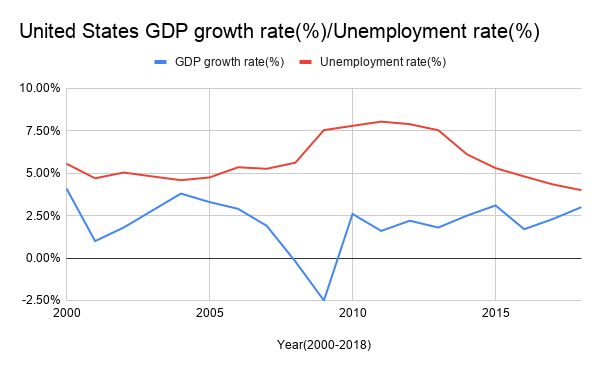
\includegraphics[scale = 0.5]{figures/United_States_GDP_Unemployment}
   \caption{Unemployment and Growth rate\cite{US_Unemployment}\cite{US_Growth_Rate_GDP}}
 \end{figure}

Here we see a somewhat clear correlation between the growth rate of the GDP growth rate and the unemployment rate of the US economy.
As seen, there is an inverse correlation between the two, meaning that when one decreases the other increases and vice versa.
If we look at the effect of the unemployment rate on the GDP growth rate in the UK it should mirror this conclusion. \\

\begin{figure}[H]
   \centering
   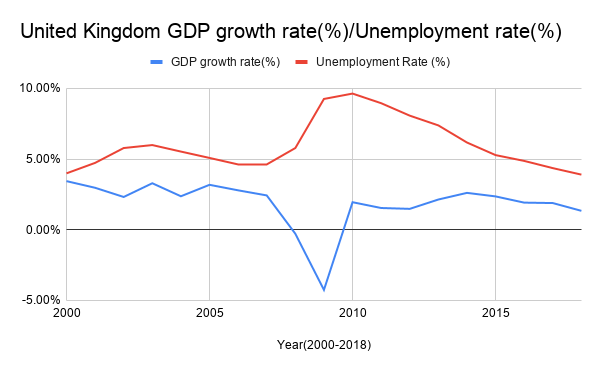
\includegraphics[scale = 0.5]{figures/United_Kingdom_GDP_Unemployment}
   \caption{Unemployment and Growth rate\cite{UK_Unemployment}\cite{UK_Growth_Rate_GDP}}
 \end{figure}

As shown, a clear inverse correlation between the growth rate of the GDP and unemployment rate can again be concluded in the UK.
This was expected and supported by the economic theory; Okun´s law.
Okun´s law states that the unemployment rate and GDP of a country have an inverse correlation.
Therefore meaning that the unemployment rate would also have an inverse effect on the growth rate of the GDP. \cite{Economics_Okuns_Law}
This correlation goes both ways, meaning that increasing the GDP growth rate of a country would decrease unemployment, and increasing the unemployment rate would decrease the GDP growth rate. \\

Now examining the correlation between the unemployment rate and wage inflation, we attempt to see if a correlation exists between the unemployment rate and wage inflation in an economy.
According to Keynesian Macroeconomic theory, there is a direct correlation:
The general economic trend is that when unemployment is high the supply of labor exceeds the number of jobs available.
So, when unemployment is high; more workers are available than jobs to fill.
Therefore, employers have little incentive to raise wages to attract workers main stagnant or decrease, and wage inflation will not occur.
However, when unemployment is low the demand for labor exceeds the number of jobs available. 
Therefore, employers now have a strong incentive to pay higher wages to attract workers, and wages will increase, and wage inflation will occur.\cite{Economics_Unemployment_Inflation}
This is all further supported by the Keynesian economic theory, the Philips curve.
The Philips curve supports the inverse correlation between the unemployment rate and inflation rate.
It states that "A Philips curve illustrates a tradeoff between the unemployment rate and the inflation rate; if one is higher, the other must be lower." \cite{Economics_Philips_Curve}
Therefore, a conclusion that being made that an inverse correlation exists between unemployment and inflation. \\

Secondly, how does unemployment affect the US and UK unemployed prospects of obtaining a job?
To better discuss the effect of unemployment let us divide unemployment into two-time frames, short-term and long-term unemployment.
Short-term unemployment defined is any unemployment period from 0 to 27 weeks, while long-term unemployment defined is unemployment 27 weeks or more. \cite{Short_Long_unemployment_Defined}
If a  can be found between the prospects of obtaining a job and unemployment, a conclusion can then be made on the effect of unemployment on the unemployed prospects of obtaining a job.

Previously, the unemployment rate was used to conclude a correlation between unemployment and the economy of the US and the UK.
However, it is problematic to make a concrete correlation between the unemployment rate and the prospects of obtaining a job for the unemployed.
This is because, as already discussed, there exists a clear correlation between the unemployment rate and the economy of a country.
Therefore, it is difficult to isolate the unemployment rate as an independent factor in an experiment, as the unemployment rate is dependent on the economy of a country and vice versa. \\

A correlation between the unemployment rate and the US and UK unemployed prospects of obtaining a job would consequently be meaningless.
As such, any conclusions made on the effect of unemployment would have to come from the status of being unemployed, not the unemployment rate.
So, is there a correlation between being unemployed and the prospects of obtaining a job in the US and UK?

Studies show a clear drop in the prospects of obtaining a job for the unemployed the longer they are unemployed.
This can be seen in the following figure, where the Federal Reserve Bank of New York conducted a study comparing the probability of finding a job and the unemployment duration in months.
The blue line representing when controlling for characteristics such as age, education, ethnicity, and gender bias, while the red represents when not taking into account characteristics.
Simply put, the study tries to isolate unemployment as a factor, making the blue line or the full controls group more reliable: \\

\begin{figure}[H]
   \centering
   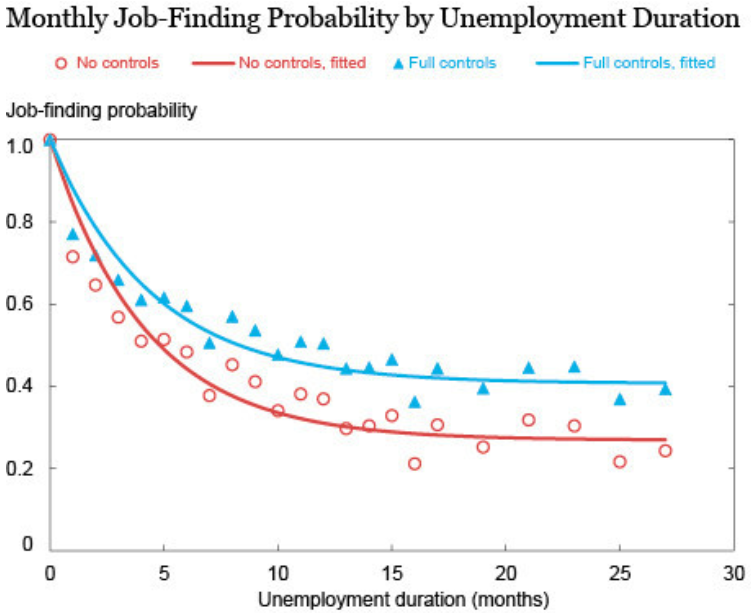
\includegraphics[scale = 0.5]{figures/Unemployment_Time}
   \caption{Unemployment and Growth rate \cite{Unemployment_effect_unemployed}}
   \label{fig:Unemployment Time}
 \end{figure}

From the figure, it can be seen that in the first eight months of being unemployed the job-finding rate falls by roughly 50\% for the controlled group and even lower for the group with no controls.
From this, we can conclude that a correlation between being unemployed and the prospects of obtaining a job exists and this correlation is affected by time.
We can similarly conclude that short-term unemployed have a rapidly decreasing probability of obtaining a job, while long-term unemployed have a stable but lowest probability of obtaining a job. 
However, it is productive to ask why this sharp decline in obtaining a job for the unemployed exists. \\
 
While many reasons could exist, a major factor is hiring personnel discrimination against the unemployed.
A study where researchers sent out the same CV only varying the length of time being unemployed found 
that "long-term unemployed workers can be up to 45 percent less likely to receive interview invitations than newly unemployed or currently employed people who look just like them".\cite{Unemployment_effect_unemployed}
This indicates that hiring personnel discrimination becomes a major factor the longer the duration of unemployment.
However, this discrimination is not always unwarranted. \\
 
A 2018 report by the National Bureau of Economic Research on discrimination of unemployed about time unemployed found that hiring personnel do not discriminate due to the status of being unemployed:\cite{Unemployment_Discrimination}
"We show that such instances are rare when firms discriminate in anticipation of an ultimately unsuccessful application. Discrimination in callbacks is thus largely a response to dynamic selection,".
Dynamic selection referring to a finding of the study that "low ability workers are more likely to be long term unemployed and duration contains information about a worker’s ability".
Therefore, hiring personnel discrimination is based on the likelihood of unemployed being less qualified, meaning that the unemployment status is not what sanctions discrimination, it is a tendency for unemployed to be less qualified.
In conclusion, unemployment has a definitive negative effect on the prospects of the US and UK unemployed prospects of obtaining a job.
These negative effects include that the probability of obtaining a job rapidly decreases for the short-term unemployed and is consistently low for the long-term unemployed.
A negative effect that is hard to deal with is the warranted discrimination of hiring personnel against all unemployed, intensifying with the duration of unemployment. \\
 
In overall conclusion, the original narrowed question posed was:
How does unemployment affect the US and UK economies and their unemployed prospects of obtaining a job?
It is possible to now answer that in terms of the unemployment effect on the US and Uk economy, unemployment has an inverse effect on the economies.
This indicates that it is in the best interest of every country to decrease the number of unemployed as this would increase economic productivity and that a.
Thereafter, it can be answered that unemployment decreases the unemployed probability of obtaining a job.
This decrease happens rapidly roughly the first six months and it is in the best interests of any country to urgently find employment for the unemployed. \\

\subsection{Obtaining a job and the process of applying for a job}
As discussed, it can become increasingly more difficult for the unemployed to get a job as time goes on.
This overlooks the discussion of the actual process of obtaining a job both for the unemployed and any other individual.
To discuss the process of getting a job, it is productive to first discuss the method by which jobs are obtained.
Thereafter, the process of applying for a job and the time frame of the process of obtaining a job.
So, how does one obtain a job and what does the process of obtaining a job look like? \\

Firstly, how do people obtain jobs?
Lou Adler, CEO of "Performance-based hiring learning systems", tried answering just this; he conducted an online survey on LinkedIn and asked how people obtained their current job.
He divided people based on job status before obtaining their current job, dividing people as variations of active or passive job searchers.
Active job searchers, as discussed in the \ref{What is unemployment and how does it materialize}, are people that have applied for a job in the prior four weeks.
He further divided active job searchers into previously unemployed and employed active searchers.
Passive job searchers are therefore anybody who has not applied to a job in the prior four weeks.
He further divided passive job searchers into tiptoers, those who passively search for other jobs without actively searching, and employed who were passively offered a job.
The results of the survey are as followed: \\

The results are outlined in \vref{fig:hiring}.
\begin{figure}[H]
   \centering
   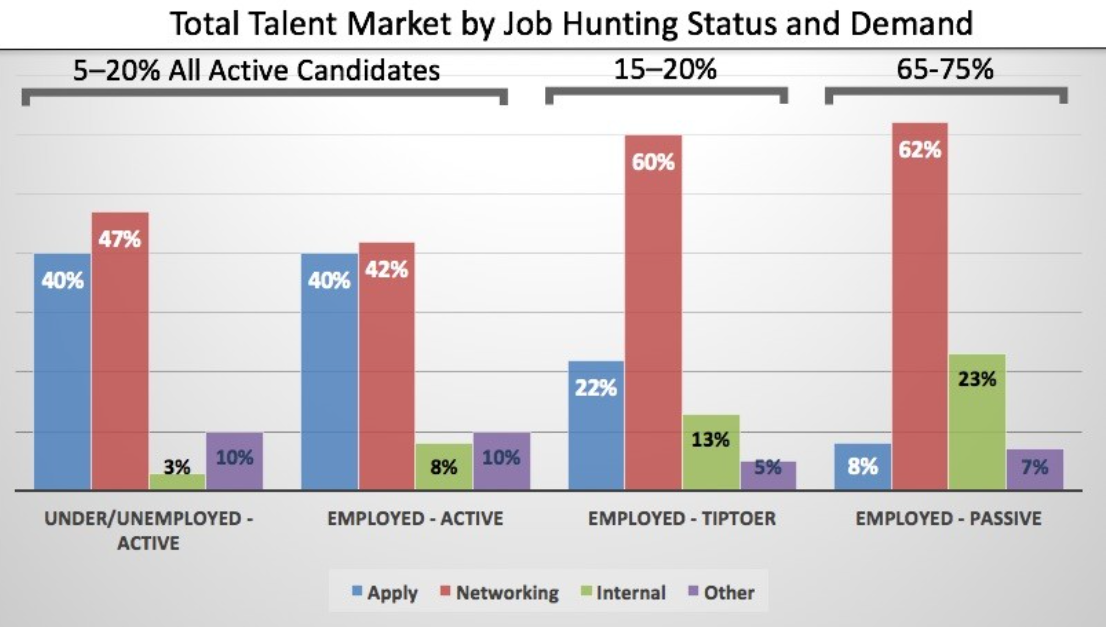
\includegraphics[scale = 0.5]{figures/hiringpeople}
   \caption{How people get jobs 2015 and 2016 \cite{Networking}}
   \label{fig:hiring}
 \end{figure}

Here we see four categories that people could be hired from. \\

The two most relevant categories are; "Apply" which would most likely be an application through CV and "Networking" which would be hiring through acquaintances or media.
From the result, we can discern that networking is the most likely factor in obtaining a job, followed by applying in most categories.
However, we see a sizable difference between the effectiveness of applying between active and passive job searchers. 
It is clear that applying has less importance for passive job searchers while applying has nearly the same effectivity as networking for active job searchers. 
This means that an effective CV process could be as beneficial for active job searchers as good networking.
But what does the process of applying to a job look like for active searchers? \\
 
The process of obtaining a job has five main stages.
These five stages are most relevant to those who apply to a firm through CV, the most likely process of application.
Although every application process is different, most firms/organizations contain these five stages.
The five stages are usually chronological and all have an obstacle that if passed lead to the next stage, ending with a job offer:
\begin{enumerate}
   \item Applying through CV to job position.
   \item ATS scanner scans your CV \cite{ATS-scanner}.
   \item Hiring personnel view you CV.
   \item Job interview with firm/organization.
   \item Job offer.\cite{Process_steps_unemployment}
\end{enumerate}
Each stage merits a discussion of the process it presents.
The first stage "Applying through CV to job position" is when an applicant sends a CV to a firm/organization.
Thereafter the CV is scrutinized by the second and third stages and is either rejected or accepted to further stages.
The second stage is the ATS(Applicant Tracking System) scanner and it scans an applicant's CV for relevant keywords based on the job position.
The third stage is the hiring personnel who will review the applicant's CV and decide which are qualified for a job interview.
The fourth stage is when the applicant is invited to a job interview, possibly more than one interview, the job/organization decides if the applicant is compatible.
In the fifth and final stage, if all previous stages are passed, the applicant is given a job offer. \\
 
But, how long can it take to get a job and how many CV´s does it take?
It is surprisingly difficult to obtain a job by applying.
A survey done by TalentWorks found that on average, when you send out an application, there is an 8.3 percent probability, that you will be invited to a job interview. 
Furthermore, on average, it takes around 10-15 interviews, before one gets a job offer. 
However, this greatly varies depending on the person, country, and economy.
However, we can conclude that on average it will take us roughly 150 applications before an applicant gets a minimum of one job offer.\cite{HR-sales} \\

This is a large amount of CV´s and can take a large amount of time to write a CV, apply to jobs, and go to job interviews.
Another factor is the time that hiring personnel takes before responding to a CV application.
For most jobs, it takes around three days before the applicant gets a response, however, for a less demanded career it can take anywhere from 10 to 30 days.\cite{HR-sales}
On average across all jobs, one can expect to hear back from employers within a week 41 percent of the time and within a couple of weeks 85\% of the time.
This means that the job process can take much longer than anticipated in most cases. \\

A study conducted by recruitment agency Randstad US surveyed 2000 Americans and found that on average it took five months to obtain a job.\cite{5_month_for_a_job}
Therefore for the average applicant, the process of applying for a job can take a lot of effort and time.
This study was not exclusively conducted on the unemployed but a mix of active searchers.
The time it takes to write a CV is another aspect.
The time can vary, based on the potential quality of the CV and applicant writing. \\
 
Sources also report contrasting time, time spent completing a CV varying from a couple of hours to several weeks.
While empirical evidence is sparse, taking a rough estimate can more accurately represent the time it takes to get a job.
An average of eight hours to write a single good CV can be found, this adds additional time for any applicant applying for a job.
Many applicants only write one CV and use it to apply to all jobs, there CV writing process taking eight hours.\cite{CV_Using_One}
However, those that choose to optimize their CV for each job they apply to will have to spend even more time and effort. \\

In conclusion, the process of obtaining a job can be strenuous and time-consuming.\cite{Time_spent_writing_CV}
As discussed it can take even longer for the unemployed to obtain a job, especially the long-term unemployed.
Therefore while five months is a better lower bounds estimate, it can easily take more than five months for the unemployed. \\

\subsubsection{ATS scanner and hiring personnel}
As discussed the process of applying for a job has five stages.
Understanding the five stages in the process of applying to a job is crucial for those applying, as 
The second and third stage, the ATS scanner and hiring personnel, both treat the first stage, that of applying with your CV.
This makes the making of the CV the most significant step in obtaining a job.
Furthermore, most applications are rejected by the ATS scanner and hiring personnel, making it the most crucial stages to pass.
Therefore, discussing the ATS scanner and hiring personnel working in more detail can give an applicant an idea of how to pass them.
So, how does the ATS scanner and hiring personnel screen an applicants CV? \\

Firstly, the ATS scanner is a keyword scanner that helps to hire personnel screen applicants, and narrow the potential candidate pool.
The ATS scanner is widely used and "70\%-80\% of large companies worldwide utilize an ATS, while smaller businesses utilize it about 50\% of the time.\cite{ATS_Usage}
Furthermore, according to Columbia University, 75 percent of applicants are phased out because their CV does not pass the ATS Scanner test.
This is a staggering amount and therefore optimizing one's CV to pass the ATS scanner is vital to obtaining a job.
In Denmark, most of the biggest companies are using ATS scanner for lessen consumed time.\cite{ATS_Denmark}

So, how does the ATS scanner screen an applicant's CV, and how does an applicant optimize their CV for the ATS scanner?
For an applicant to optimize their CV for the ATS scanner, the way the ATS scans an applicant's CV must be discussed.
Many versions of ATS scanners also exist, with the most widely used being the iCIMS, Bullhorn, Taleo, and Greenhouse.
While no two are the same, they all scan for the same underlying elements in an applicants CV:
\begin{enumerate}
   \item Scan education
   \item Scan work experience
   \item Scan relevant keywords throughout CV
\end{enumerate}
However, how does the ATS scanner scan for these elements in a CV?
All ATS scanners have slightly different methods, so, therefore, it is productive to use Taleo, the most widespread ATS scanner as a template example.
The Taleo ATS scanner works by having pre-defined keywords chosen by the firm/organization, that it then searches for in the applicants CV´s.\cite{ATS_Taleo}
The most constructive way to discuss the working of Taleo's ATS scanner is to have an example scenario. \\

A scenario could be a shipping company, that is searching for a candidate with a bachelor, that also has work experience with programming and has leader characteristics, they will have "bachelor", "programmer" and "leader" as pre-defined keywords.
Taleo will then search through every applicant's CV´s for the keywords "bachelor", "software" "leader".\cite{ATS_Purpose_Workings}
Often Taleo will categorize a CV based on the headers established by the applicant in the CV.
The shipping company will most likely give instructions to Taleo to only search for the keywords "bachelor" under the header "education".
Therefore eliminating any random occurrence of the word out of the context of education. \\

A firm/organization can also set the importance of certain pre-defined keywords through Taleo.
Some pre-defined keywords may be awarded a system of points for how often they appear in an applicant's CV, or some words may be required by Taleo.
Meaning that if certain pre-defined keywords do not appear in the applicant's CV, then the CV is rejected. \\

Taleo along with all modern ATS scanners can recognize synonyms and therefore small deviation from the pre-defined keywords may not be fully penalized.
If the shipping company´s ATS scanner scans a CV and finds the word "director", it may award the points equal to or a fraction of "leader".
If an applicant's CV contains all the required keywords, then the points are added and ranked among the other CV´s.
Hiring personnel tends to consider those CV´s with the highest ranking, so it is preferable to rank as highly as possible. \\

The ATS scanner can seem a nuisance for applicants, as the firm/organization selects the predefined keywords and the applicant has to guess which keywords to include in their CV.
Furthermore, a study by career arc found that " 62\% majority of employers who use applicant screening tools admit that some qualified candidates are likely being automatically filtered out of the vetting process by mistake".\cite{CV_ATS_Broken_System}
This points to the ATS scanner is potentially a flawed system, screening qualified applicants and allowing less-qualified applicants through.
As discussed, most applicants only write one CV, partly because it can be extremely time-consuming if an applicant wishes to create a CV optimized for the ATS scanner for each and every job they apply to.
However, the ATS scanner's purpose is to screen those that are not qualified, in this it is predictable and can be systematically be overcome.
A CV that contains the right keywords and structure should be both in the interest of the firm/organization and applicant, to pass and rank highly on the ATS scanners list. \\

Secondly, as discussed, after all, CV´s have been screened by the ATS scanner, the hiring personnel views that CV´s not rejected by the ATS scanner.
The method by which they scrutinize the applicant's CV´s varies, much like the ATS scanner.
Understanding the method by which the hiring personnel view applicant's CV´s can aid applicants in passing the hiring personnel stage, thereafter being invited to a job interview.
Unlike the ATS scanner, which is predictable in its systematic scanning. 
Hiring personnel inserts a human element and therefore an unpredictability.
However, some general trends can still be made about how hiring personnel screen applicants CV. \\

According to the majority of studies, hiring personnel spend 5 to 9 seconds (depending on the study) considering an applicant's CV, if the CV does not appeal in this small time frame, the CV will be rejected.
This means that the first impression is vital to the success of passing the hiring personnel and warranting a job interview.
James Reed is the author of the book "The 7 Second CV" and has written three other books on the job interview process.\cite{7_second_test}
According to James Reed, most hiring personnel will only spend 7 seconds on each CV, and that a CV must be able to stand out in those first 7 seconds. \cite{7_Seconds_to_Get_a_Recruiter_Attention} \\
James Reed book puts much emphasis on the following concepts:
\begin{enumerate}
   \item Accessibility to content 
   \item Content relevance
   \item Wording of content
\end{enumerate}\cite{7_second_test}
It is vital to discuss each concept and what does it entail.
Accessibility to content highlights the need for a good first impression.
The structure and content of a CV must invite further study, it must catch the hiring personnel's interest.
The CV must also be of a length in which the hiring personnel does not reject the CV based on assumptions.
If the CV is too short the hiring personnel may regard the applicant as under-qualified.
Furthermore, if the CV is too long the hiring personnel may regard the CV as incomprehensible and disorganized. \\

According to a survey by TalentWorks that analyzed 6000 job applications the optimal length for a CV is 475-600 words.\cite{CV_Word_length}
These should be enough words to convey the necessary content to the hiring personnel effectively. 
However, arguably number of pages is what leaves a stronger impression on the hiring personnel.
CareerAddict outlines the optimal number of A4 pages in most cases as being based on applicant:\cite{CV_Page_length}
"One-page CVs are best for school leavers, recent graduates, and generally early jobseekers who have little to no professional experience at all."\cite{CV_Page_length}
While two pages are "preferred by 91\% of recruiters", CareerAddict claims many companies "reject CVs that are less than two pages because they simply don’t provide enough evidence about the applicant’s skills and qualifications".\cite{CV_Page_length}
Three pages are generally used only by executives or academics that have a long list of qualifications.
Therefore, the most accessible length of a CV for most applicants is two pages with 475-600 total words. \\

The next concept is content relevance and it can be difficult as it pertains to each applicant's CV differently.
As the first impression is everything to passing the hiring personnel, the content must be immediately conveying a sense of qualification.
Therefore, meaningless content and content that can not stand alone apart from other content must be discarded to optimize a CV for passing the hiring personnel.
The wording of content pertains to the method with the CV addresses the applicant.
Implementing the keywords to optimize for the ATS scanner will fill the same objective with the hiring personnel.
As the CV will look more relevant to the job position for the hiring personnel.\\

\subsection{Required and situational content of a CV}
As discussed, the content of a CV is crucial to passing both the hiring personnel and ATS scanner.
However, what is a CV in actuality, and what is required content for a CV to contain.
Furthermore, as each application has different qualifications, each applicant's CV must-have content situationally purposed for their CV.
Therefore, what is a CV and what is the required and situational content of a CV? \\

A CV is “a short account of one’s career of qualifications prepared typically by an applicant for a position”.\cite{Difference_between_resume_and_curriculum_Vitae}
When applying for a position within a firm, some aspects of a CV are required.
These requirements can come from the position or firm that the CV is intended for or from the definition of the CV itself.
Putting aside the firms or positions requirements, all CVs must include the five following requirements to be defined as a CV:
\begin{itemize}
   \item 1. Contact information
   \item 2. CV objective
   \item 3. Relevant skills
   \item 4. Work experience
   \item 5. Education\cite{Write_a_curriculum_Vitae} \\
\end{itemize}
The substance of each requirement varies from applicant to applicant. However, every CV must include these five requirements to be effective.
A further explanation of each requirement is due:
Contact information is required as the firm at the bare minimum must have some way to contact the person so he or she can be accepted for the position.
CV objective is required as it specifies what and who the CV is intended and without it, the CV can fill no purpose.
Relevant skills are required as without them you have no relation to the CV objective.
Work experience and education are required as without it one has no qualifications. \\

As a CV is an account of one’s qualifications it is also possible to leave education and work experience empty if one has none.
However, it is then hardly an effective CV.\cite{Difference_between_resume_and_curriculum_Vitae}
Along with the requirements of a CV, there are also aspects that are situational.
These vary and most likely the firm or position to which one is applying will lay out these aspects, or it is apparent from the position itself.
If not specified it is difficult to know what to include. Too little and one will under-qualified, too much and the CV will be too long.\cite{Job_Application_for_science}, excesses and unorganized.
Therefore, it is essential to distinguish one’s CV with the right quantity and quality of situational content.
Let's examine some of the more typical situational content that could be included in a CV: \\
\begin{itemize}
   \item 1. Professional association
   \item 2. Volunteer experience
   \item 3. Languages
   \item 4. Additional training courses
   \item 5. Publication
   \item 6. Awards/Honors
   \item 7. References\cite{6_sections} \\
\end{itemize}
The effectiveness of a CV can drastically change due to use of situational content.
Therefore it is necessary to further explain each situational content: \\
Professional association is any trade unions, learned societies, regulatory universities and other inter-professional societies.
Many associations have certain prestiges and hold there member to a certain standard of quality.
Therefore a professional association can improve a CV if relevant.\cite{Professional_associations_and_organizations}\cite{Perks_of_professional_organizations}
Volunteer experience is any volunteer work relevant to the position.
Languages is any spoken or written language relevant to the position.
As most firms in our interconnected market interact with some multilingualism, languages can easily increase the quality of a CV.
Additional training courses are any extra courses relevant to the position. 
Publication are any reports, books or other published materials that could show qualifications for the given position.
Awards and honors are any university or professional awards or honors given that show qualification for thr given position.
References are very situational, as putting references in a CV may make you seem unsure of yourself and in need of validation from others to show qualifications.
However, if a CV has the right references it can assure employers of your qualifications and past experience. \\

\subsection{Structure of the CV}
As discussed, the structure of a CV is crucial to passing both the hiring personnel and ATS scanner.
Writing an effective CV isn't just about including the right content. 
It's also about how you present that information.
Structure is vital to leaving a good first impression upon the hiring personnel.
Furthermore, the structure of a CV must allow the ATS scanner to find the correct keywords in the headers. 
As such, the structure of an applicants CV is essential to obtaining a job.
Therefore, what are the possible structures of an applicants CV and does a optimal structure exist to obtaining a job? \\


Every applicant must have a structure that best presents their CV.
It is therefore relevant to discuss the different structures available to the applicant. 
In theory, an applicant could structure their content in a million different ways.
To narrow it down we will not discuss the three most common structures and the pros and cons of each of them.

The first structure is the Chronological CV structure: \\
\begin{itemize}
   \item  Contact information
   \item  CV objective
   \item  Work experience
   \item  Education
   \item  Relevant skills
   \end{itemize}
The Chronological CV structure is the most common and gives an easy overview of the applicant's content.
It is adaptable and features all required content mentioned in (Required and situational content of a CV).
With the added section "relevant skills" where the applicant can include their situational content to standout.
Its traditional structure is simple for both hiring personnel and the ATS Scanner to view.
The structure is best suited for those who are confident in their CV content, especially their work experience and education.
The structure can have a difficult standing out as it is the most common and should not be used by those who have big gaps in employment.\\
   
The second structure is the Functional CV structure:
\begin{itemize}
   \item  Contact information
   \item  CV objective
   \item  Relevant skills
   \item  Situational content
   \item  Work experience
   \item  Education\\ 
   \end{itemize}
The Functional CV structure focuses on relevant skills and situational content over work experience.
This structure is favored by those applicants with large gaps in their unemployment history, or in the middle of a career change.
As the structure emphasizes the applicant's relevant skills and situational content it is flexible as the applicant has a chance to present himself on his terms.
This structure is highly dependant on the applicant's relevant skills and how they present their significance to the job they are applying for.
The structure is highly flexible and can either be a nightmare for both the hiring personnel and ATS scanner or if structured correctly with correct usage of keywords be highly effective.\\
    
The third structure is the Combination CV structure:
\begin{itemize}
   \item  Contact information
   \item  CV objective
   \item  Relevant skills
   \item  Work experience
   \item  Situational content
   \item  Education \\
   \end{itemize}
The Combination CV structure is as stated, a combination of the Chronological and Functional CV structures. 
It enables the applicant with otherwise mediocre content to combine the two and compensate for a weakness with another CV structure.
This is a highly flexible structure and lets an applicant who knows how to present oneself to standout.
It is not a structure that an applicant with either overwhelming relevant content or no relevant content to users.
   As the structure does not allow for a high emphasis on one section without an obvious lack in the others.
   \cite{Resume_structure}
   \cite{Tips_for_best_format}
   \cite{8_Best_cv_format}
\clearpage
